% % $RCSfile: proj_proposal.tex,v $
% % $Revision: 1.3 $
% % $Date: 2016/06/10 03:44:08 $
% % $Author: kevin $

\documentclass[11pt, a4paper, twoside, openright]{report}

\usepackage{float} % lets you have non-floating floats
\usepackage{url} % for typesetting urls

\renewcommand{\thesection}{\arabic{section}}

%  We don't want figures to float so we define
%
\newfloat{fig}{thp}{lof}[chapter]
\floatname{fig}{Figure}

% % These are standard LaTeX definitions for the document
% %
\title{Instrumentation System for Liquid Drop Impact and Evaporation \\ 8 pages MAX}
\author{Daniel Eisen}

% % This file can be used for creating a wide range of reports
% %  across various Schools
% %
% % Set up some things, mostly for the front page, for your specific document
%
% Current options are:
% [ecs|msor|sms]          Which school you are in.
%                         (msor option retained for reproducing old data)
% [bschonscomp|mcompsci]  Which degree you are doing
%                          You can also specify any other degree by name
%                          (see below)
% [font|image]            Use a font or an image for the VUW logo
%                          The font option will only work on ECS systems
%
\usepackage[image,ecs]{vuwproject} 

% You should specifiy your supervisor here with
\supervisor{Gideon Gouws}
% use \supervisors if there are more than one supervisor
\otherdegree{Bachelor of Engineering with Honours}
% Unless you've used the bschonscomp or mcompsci
%  options above use
%   \otherdegree{OTHER DEGREE OR DIPLOMA NAME}
% here to specify degree

% Comment this out if you want the date printed.
\date{}

\begin{document}

% Make the page numbering roman, until after the contents, etc.
\frontmatter

% %% %% %% %% %% %% %% %% %% %% %% %% %% %% %% %% %% %% %% %% %% %% %% %% %% %% %%

\begin{abstract}
    This document gives some ideas about how to write a project
    proposal, and provides a template for a proposal. You should discuss
    your proposal with your supervisor.
\end{abstract}

% %% %% %% %% %% %% %% %% %% %% %% %% %% %% %% %% %% %% %% %% %% %% %% %% %% %% %%

\maketitle

\tableofcontents

% we want a list of the figures we defined
%\listof{fig}{Figures}

% %% %% %% %% %% %% %% %% %% %% %% %% %% %% %% %% %% %% %% %% %% %% %% %% %% %% %%

\mainmatter

% %% %% %% %% %% %% %% %% %% %% %% %% %% %% %% %% %% %% %% %% %% %% %% %% %% %% %%

\section{Introduction}

\section{The Problem}
This project is concerned with the development of a instrumentation rig for the study of droplet impact and drying. It is primarily/initially motivated by the powdered milk production process, specifically the behaviour of the drying and collision of concentrated milk droplets. Furthermore, the research, and developed method and procedure can be applicable to various industries. \\

To effectively investigate the behaviour, a variety of aspects can be tracked and characterised during a microscale equivalent lab process, from differing temperatures, substrates, volume, and concentrations. \\

Currently there is an existing platform for the dispensing of droplets and data capture using high speed cameras and other various sensors. It

This project will therefore, focus on the design and evaluation of the third generation of this platform with the aim to design and integrate various new subsystems and evaluate their performance against the criteria of improving the reliability and repeatability of the experiments as much as possible.



\section{Proposed Solution}

Evaluate current systems results and identify its short comings. Produce evaluation data and bibliography (est. x wks)
\begin{itemize}
    \item Repeatability of [Drop position,Drop volume (size),Contact angle] and correlate and/or see how the variation in these parameters effects the observed temperature profile and physical behaviours of the droplet throughout the evaporation process.
    \item Identify other sources of variation, such as humidity etc and their weight of influence (whether perusing a solution is worthwhile)\\
    \item Compare with similar solutions in literature to gain more insight into required design consideration and constraints.
\end{itemize}

\subsection{Milestones}
\begin{itemize}
    \item
    \item
    \item
\end{itemize}

\subsection{Timeline}
\begin{figure}[h]
    \centering
    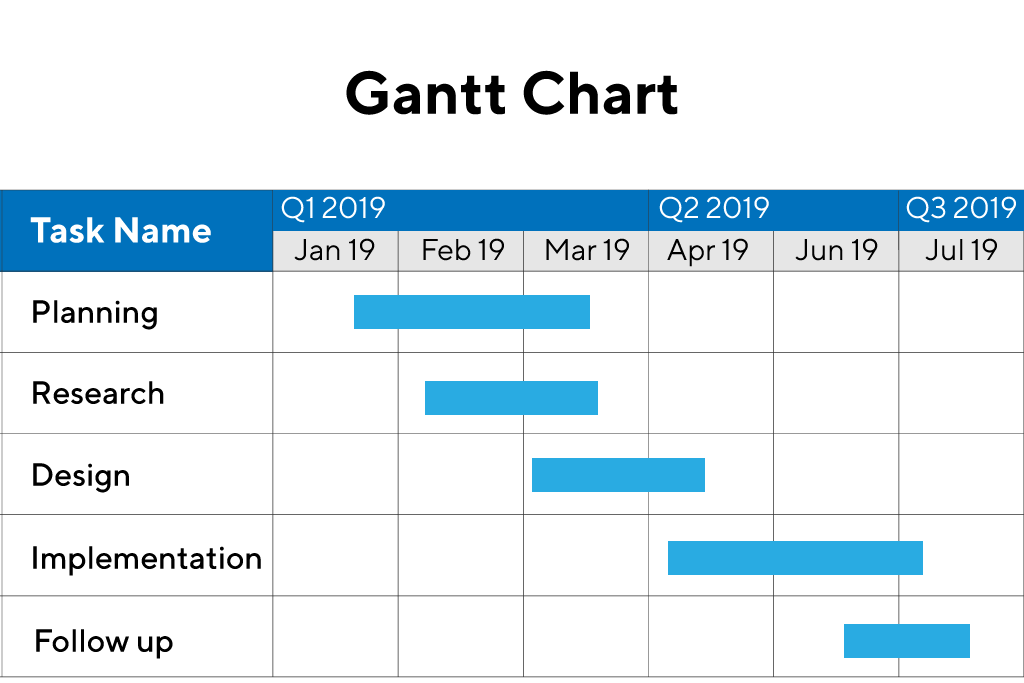
\includegraphics[width=0.5\textwidth]{Figures/Gantt-chart_filler.png}
    \caption{Example Gantt Chart filler, will be replaced with actual timeline}
\end{figure}

\section{Evaluating your Solution}



\section{Resource Requirements}

\subsection{Facilities and Tools}
\begin{itemize}
    \item Labs AM219 and LB207
    \item Computer with SolidWorks, LabView, \textit{other data processing tools}
    \item Electronics Test bench (PSU, signal gen, scope etc)
    \item Access to fab workshop
\end{itemize}

\subsection{Budget }

\subsection{COVID Alert Level Management}
Level and planned work that can be achieved and undertaken at the various levels.
\subsubsection*{Level 1}
\subsubsection*{Level 2}
\subsubsection*{Level 3}
\subsubsection*{Level 4}


% %% %% %% %% %% %% %% %% %% %% %% %% %% %% %% %% %% %% %% %% %% %% %% %% %% %% %%
\backmatter
% %% %% %% %% %% %% %% %% %% %% %% %% %% %% %% %% %% %% %% %% %% %% %% %% %% %% %%

\nocite{*}
\bibliographystyle{ieeetr}
\bibliography{sample}
\end{document}
